\documentclass[tikz,border=10pt]{standalone}
\usepackage{tikz}
\usetikzlibrary{arrows.meta, positioning}

\begin{document}

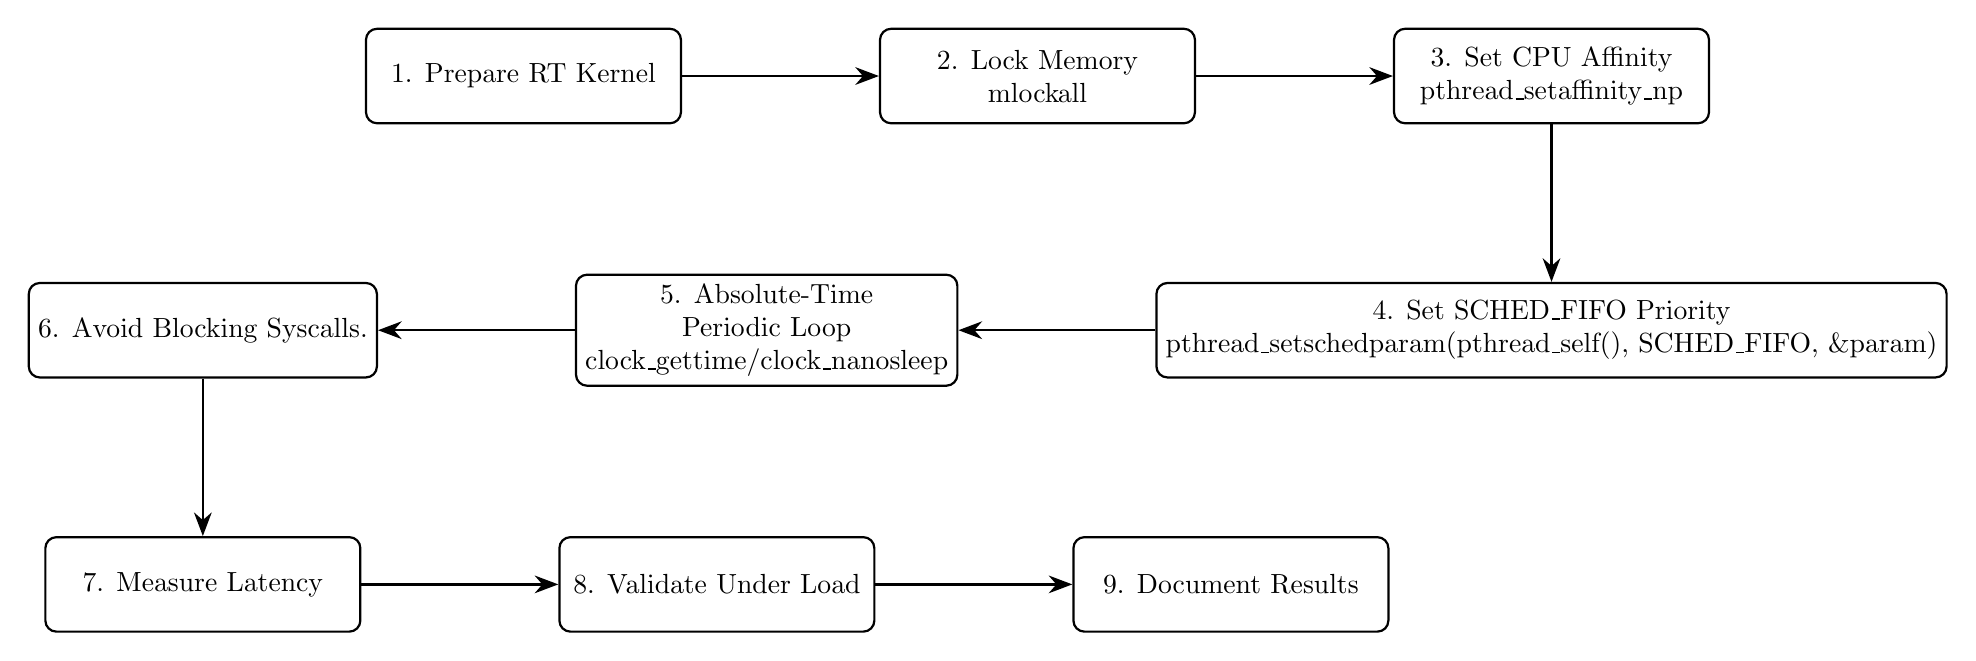
\begin{tikzpicture}[
    node distance=2cm and 2.5cm,
    box/.style={
        rectangle,
        draw,
        thick,
        rounded corners,
        align=center,
        minimum width=4cm,
        minimum height=1.2cm
    },
    arrow/.style={
        -{Stealth[length=3mm]},
        thick
    }
]

% --- Row 1 (Left to Right) ---
\node[box] (n1) {1. Prepare RT Kernel};
\node[box, right=of n1] (n2) {2. Lock Memory \\ mlockall };
\node[box, right=of n2] (n3) {3. Set CPU Affinity \\ pthread\_setaffinity\_np };

% --- Row 2 (Right to Left) ---
\node[box, below=of n3] (n4) {4. Set SCHED\_FIFO Priority \\ pthread\_setschedparam(pthread\_self(), SCHED\_FIFO, \&param)};
\node[box, left=of n4] (n5) {5. Absolute-Time\\Periodic Loop \\ clock\_gettime/clock\_nanosleep};
\node[box, left=of n5] (n6) {6. Avoid Blocking Syscalls.};

% --- Row 3 (Left to Right) ---
\node[box, below=of n6] (n7) {7. Measure Latency};
\node[box, right=of n7] (n8) {8. Validate Under Load};
\node[box, right=of n8] (n9) {9. Document Results};

% --- Arrows Row 1 ---
\draw[arrow] (n1) -- (n2);
\draw[arrow] (n2) -- (n3);

% Down turn
\draw[arrow] (n3) -- (n4);

% --- Arrows Row 2 (Right to Left) ---
\draw[arrow] (n4) -- (n5);
\draw[arrow] (n5) -- (n6);

% Down turn
\draw[arrow] (n6) -- (n7);

% --- Arrows Row 3 ---
\draw[arrow] (n7) -- (n8);
\draw[arrow] (n8) -- (n9);

\end{tikzpicture}

\end{document}
